\section{ИССЛЕДОВАНИЕ РАБОТЫ D-ТРИГГЕРА}

\begin{figure}[H]
	\centering
	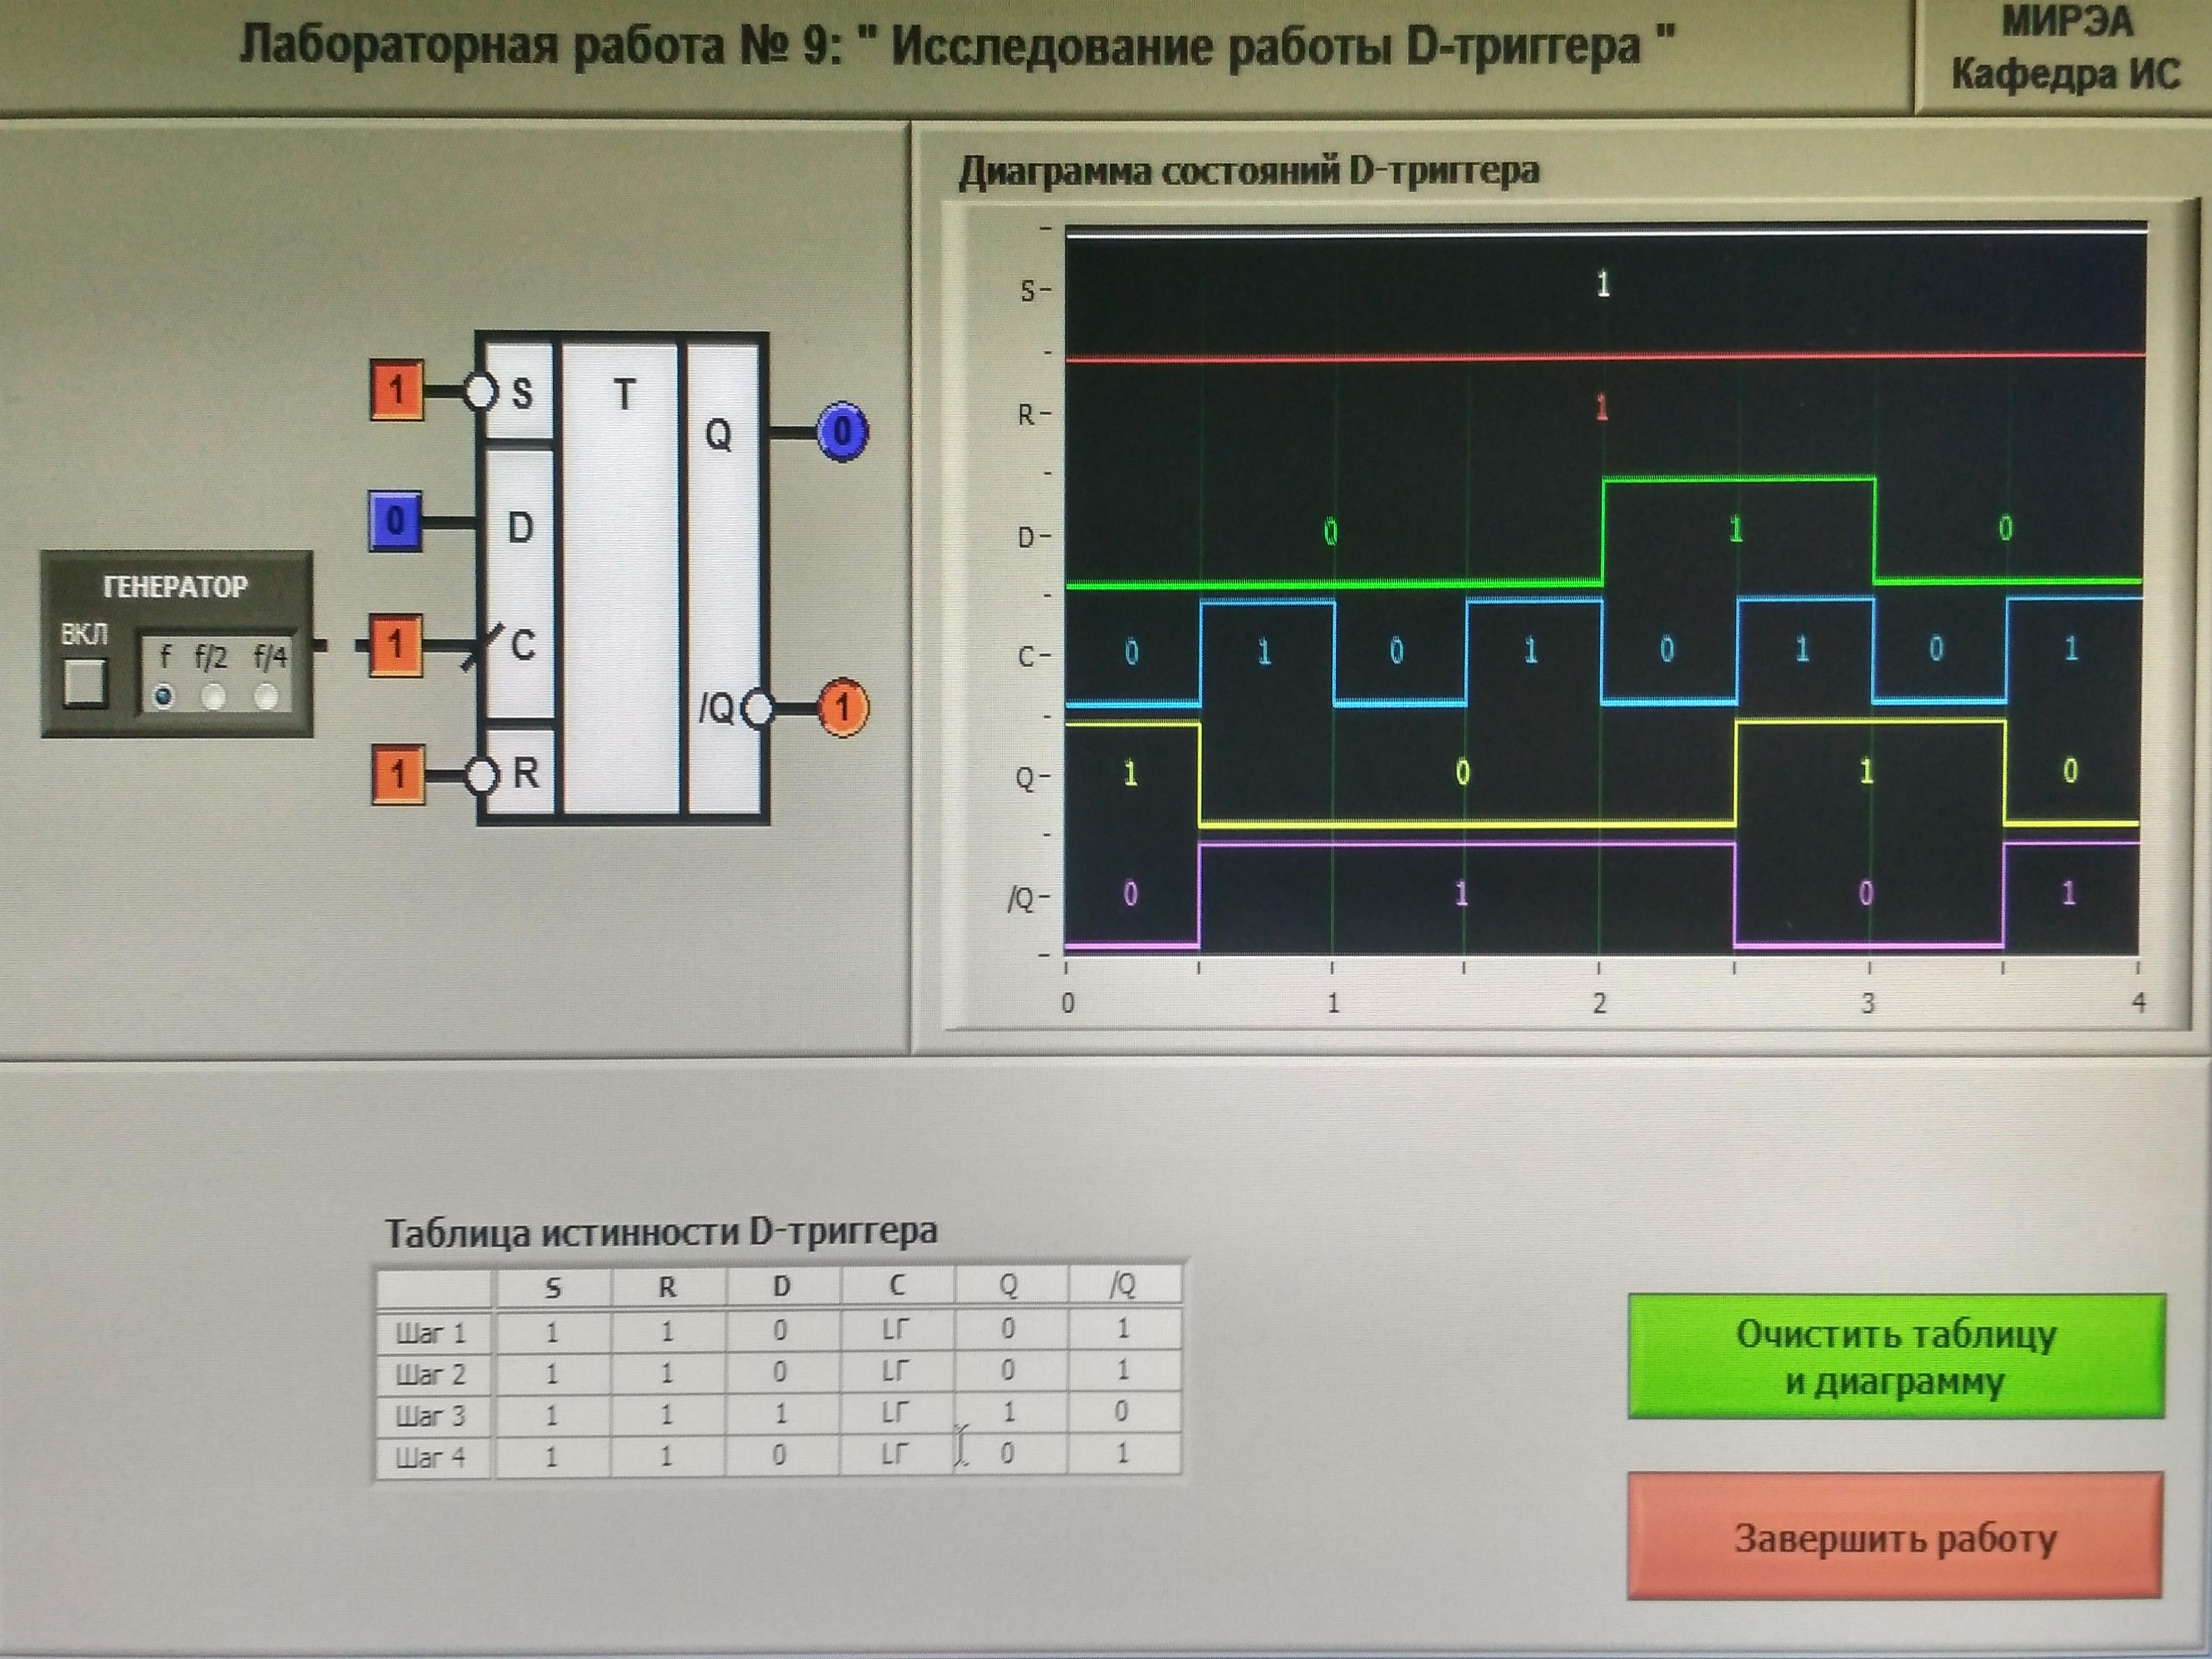
\includegraphics[width=0.95\linewidth]{imgs/9/1}
	\caption{Результат работы D-триггера}
	\label{fig:9_1}
\end{figure}

\begin{table}[H]
	\centering
	\caption{Переключение состояния D-триггера}
	\label{tab:lab_09_states}
	\begin{tabular}{|c|c|c|}
		\hline
		Выход $Q_n$ & Вход D & Выход $Q_{n+1}$ \\ \hline
		0           & 0      & 0               \\ \hline
		0           & 1      & 1               \\ \hline
		1           & 0      & 0               \\ \hline
		1           & 1      & 1               \\ \hline
	\end{tabular}
\end{table}

\begin{table}[H]
	\centering
	\caption{Список состояний D-триггера}
	\label{tab:lab_09_mode}
	\begin{tabular}{|c|c|c|}
		\hline
		Режим работы        & Вход D \\ \hline
		Установка 1         & 1      \\ \hline
		Установка 0         & 0      \\ \hline
	\end{tabular}
\end{table}

\begin{figure}[H]
	\centering
	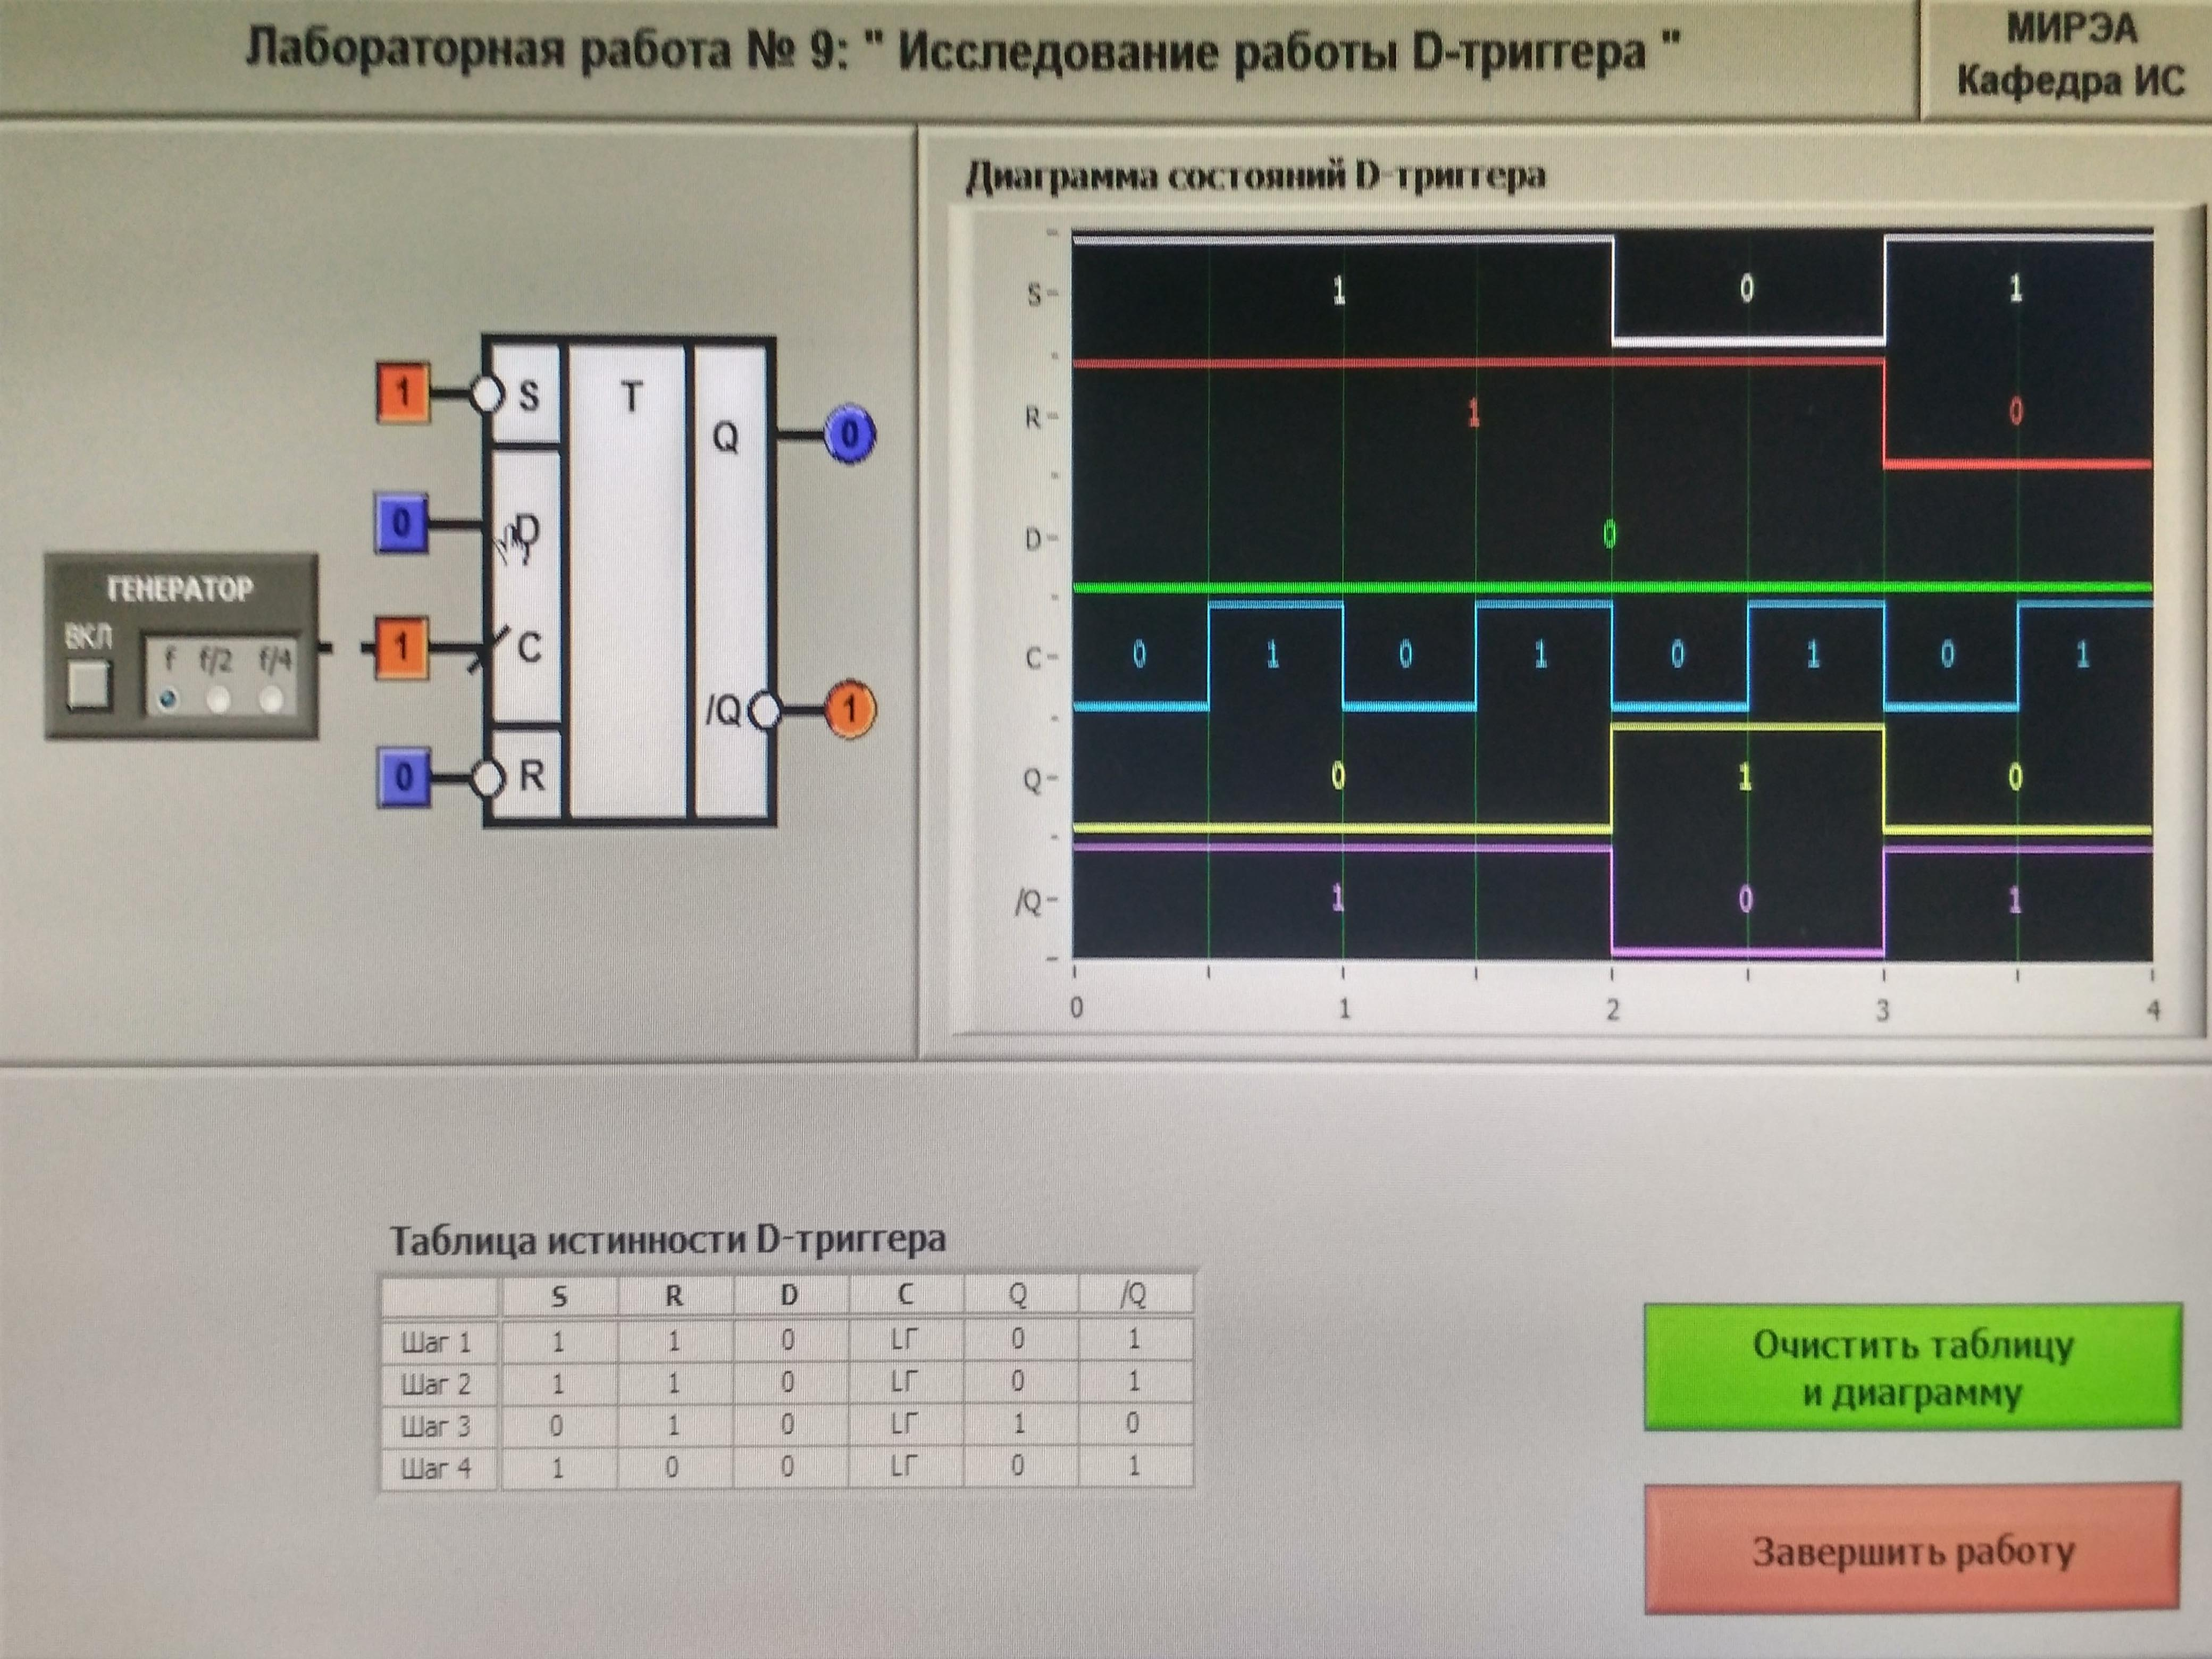
\includegraphics[width=0.95\linewidth]{imgs/9/2}
	\caption{Результат работы D-триггера в режиме генератора}
	\label{fig:9_2}
\end{figure}

Активный уровень сигнала для входов RS - низкий.
При подаче низкого активного сигнала входы JKC влияния не оказывают.
Переключение состояние триггера происходит при переходе состояния C с низкий уровня на высокого.

Элемент SN74HCS72-Q1 - High-Speed CMOS

Характеристики:

\begin{figure}[H]
	\centering
	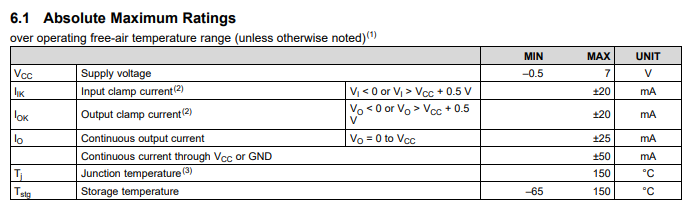
\includegraphics[width=0.95\linewidth]{imgs/9/ti1}
	\caption{Максимальные рабочие параметры}
	\label{fig:9_ti1}
\end{figure}

\begin{figure}[H]
	\centering
	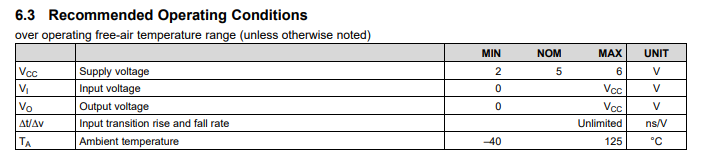
\includegraphics[width=0.95\linewidth]{imgs/9/ti2}
	\caption{Рекомендуемые параметры}
	\label{fig:9_ti2}
\end{figure}

\begin{figure}[H]
	\centering
	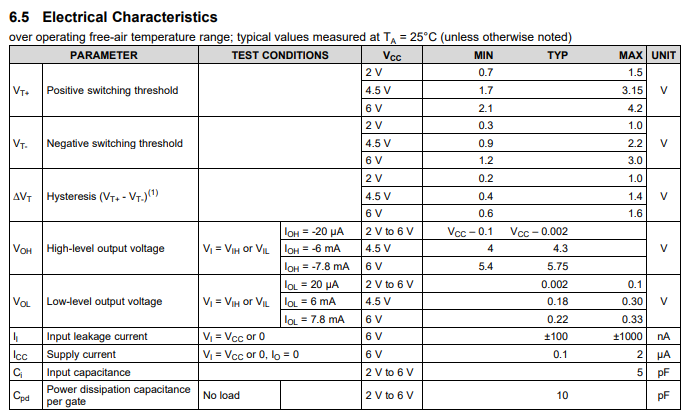
\includegraphics[width=0.95\linewidth]{imgs/9/ti3}
	\caption{Электрические характеристики}
	\label{fig:9_ti3}
\end{figure}

\begin{figure}[H]
	\centering
	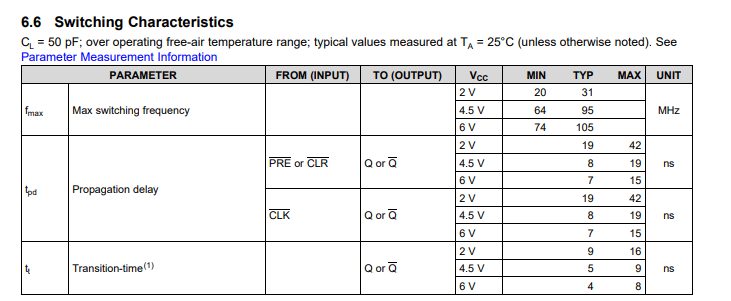
\includegraphics[width=0.95\linewidth]{imgs/9/ti4}
	\caption{Характеристики переключения}
	\label{fig:9_ti4}
\end{figure}

\begin{figure}[H]
	\centering
	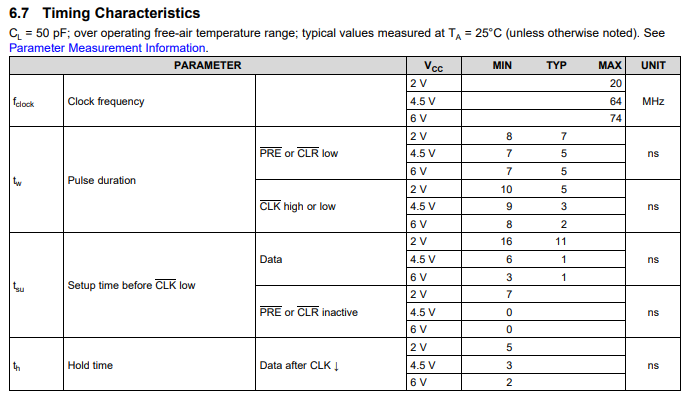
\includegraphics[width=0.95\linewidth]{imgs/9/ti5}
	\caption{Временные характеристики}
	\label{fig:9_ti5}
\end{figure}